\chapter{The App System: making it intelligent}
\label{apps}

\zway operates on two levels: Every function of the device in the network will be shown 
as an element. Elements are shown automatically but can be deactivated or hidden. All 
other functions are realized and managed in apps. These apps can be grouped into four categories.

\begin{enumerate}
\item More elements that use services and information from the Internet or other 
TCP/IP-connected devices from third parties. Examples of this include weather information 
taken from online weather services or the control of a SONOS music system. There are also 
settings for out-of-band communication to users utilizing push notification, email, 
SMS, and voice output.
\item Logical connections between elements and other services. This is usually referred 
to as automation. It connects element functions with each other or with timer information. 
Example are a time-driven control of lights, heating, or turning on or off the light based 
on a motion detector.
\item Connection and integration of third-party smart home systems and technologies. One 
of the most commonly known systems is Apple Homekit. Other systems are openremote.org, 
IFTTT, etc.
\item A big number of apps is needed to unlock special functions of physical devices 
(or fix-specific bugs). Examples are the control of user codes and user accesses of a 
keypad or special displays of energy consumption that are not done by \zway by default.
\end{enumerate}

Some important apps are already pre-installed on \zway. Most of the apps are available 
online on the server and need to be downloaded before they can be used. This chapter 
gives some examples and recommendations for typical apps available.

\section{A simple Apps as starter - \app{Local Weather}}

\begin{figure}
\begin{center}
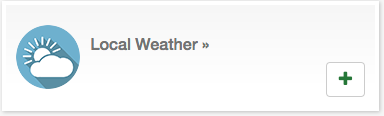
\includegraphics[width=0.4\textwidth]{pngs/cap6/app5.png}
\caption{The Open Weather app in the App Repository}
\label{app5}
\end{center}
\end{figure}

\begin{figure}
\begin{center}
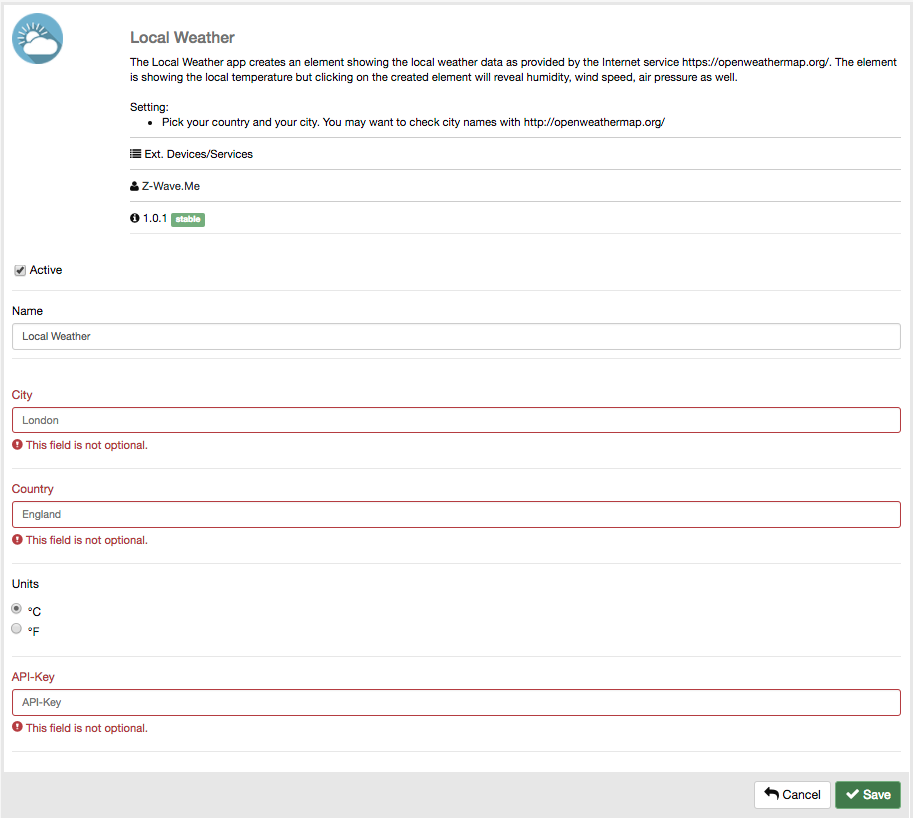
\includegraphics[width=0.7\textwidth]{pngs/cap6/app6.png}
\caption{The Open Weather app configuration}
\label{app6}
\end{center}
\end{figure}


Displaying the local weather inside the smart home user interface is a simple and popular 
task. \zway offers several apps for this request. Already on the device you fine the 
app \app{Local Weather} calling data from the known service openweather.org. The 
data is provided free of charge; however, an API key is needed to access the data. 
Visit www.openweather.org and register as a user to access your API key. After that, 
install the weather app \app{Local Weather} (see Figure \ref{app5}) from the local 
app repository. Figure \ref{app6} shows the configuration dialog:

\begin{enumerate}
\item Rename the app to your own needs
\item Pick the name of the city
\item Pick the country of this city (agreed this is foolish, but this is how openweather accepts data)
\item Choose between Celsius and Fahrenheit
\item Insert the API key received from openweather.org
\end{enumerate}

Once activated, a new element is shown on the element view displaying the temperature 
and the weather situation. Clicking on the small triangle on the right-hand side opens 
a small window with more weather information such as air pressure, wind speed, relative 
humidity. The data is updated hourly.

It is possible to display certain values as single element in the element view. This can 
then be used for automation. Please note, that both the IF and the THEN side of automation 
like \app{IF->THEN} must always refer to active elements. for more information about the 
\app{IF->THEN} app please refer to Chapter \ref{cap:ifthen}.

An interesting app is \app{Virtual Rain Sensor}. This app creates an app indicating if it 
was raining on the location. This app sits on top of a weather app and uses their 
functions and setup. This example shows that certain apps can depend on other apps 
to be installed first. This concept is known from PC software where certain applications 
require certain tools or libraries installed first.

\section{Smart Home Logic}

Logic or automation is the core of the Smart Home. It allows doing things automatically 
depending on certain conditions.

\subsection{Scene}
\label{sceneapp}

\begin{figure}
\begin{center}
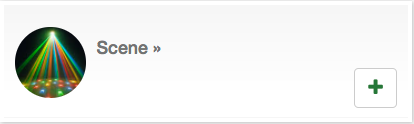
\includegraphics[width=0.4\textwidth]{pngs/cap6/app7.png}
\caption{The Scene App}
\label{app7}
\end{center}
\end{figure}


The most basic step to simplify life is to group multiple actions into one action. There 
is no need to have a smart home controller in the home to do this. Even classical electrical 
wiring allows switching on two lights with one switch. However, smart home allows 
creating much larger actions just triggered with one (virtual or real) button. The tool
for this is called \app{Scene} and the app is shown in Figure \ref{app7}.

The configuration of the scene app is quite straightforward. All devices to be controlled 
with the ``one button’’ need to be identified and their desired switching status defined.

The scene itself becomes a virtual device, which is why it is also possible to create 
a hierarchy of scenes and to let one scene switch the other scene.

\begin{figure}
\begin{center}
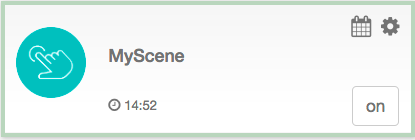
\includegraphics[width=0.4\textwidth]{pngs/cap6/app8.png}
\caption{The Scene Element}
\label{app8}
\end{center}
\end{figure}

Once stored, there is a new element with the name of the scene as shown in Figure \ref{app8}. 
There is only one button to turn on the scene. A scene can never be turned off but only 
replaced by a different scene. The reason for this is that it is not reasonable to turn 
back to the previous state, since individual devices of the scene may have been operated 
in the meantime. The scene element shows the time stamp when this scene was activated 
the last time. The event history shows all the events (activations) the scene, much 
like how it is done on any other \zway actuator.

\begin{figure}
\begin{center}
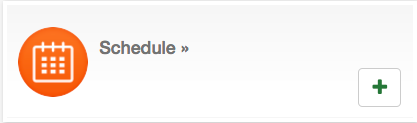
\includegraphics[width=0.4\textwidth]{pngs/cap6/app9.png}
\caption{Schedule - an scheduled Scene}
\label{app9}
\end{center}
\end{figure}

An enhancement for the scene app is the \app{Scheduled Scene} or \app{Schedule}, as shown in 
Figure \ref{app9}. This app combines the scene function with a simple weekly calendar that 
allows executing the scene at a special time per day.


\subsection{If -> Then}
\label{cap:ifthen}

The most basic relationship of automation is the If->Then relationship

\paragraph{Some examples}
\begin{quote}
\textbf{IF} button 2 on the remote control is pressed, \textbf{THEN} the ceiling 
lamp will turn on. \textbf{IF} temperature sensor goes above $22^\circ C$, $\rightarrow$ 
\textbf{THEN} turn down the heating \textbf{AND} open the window.
\end{quote}

In order to accomplish this kind of IF$\rightarrow$ THEN relationship the following 
requirements need to be met:

\begin{itemize}
\item The actor device needs to be identified and able to perform the desired task.
\item The sensor or controller needs to be able to generate an event that causes the action.
\item The sensor or controller needs to know which actor to control and in which way in 
case of an event.
\end{itemize}

The first requirement is quite obvious. If the ceiling light---to stay in the first 
example---is turned on, the ceiling light needs to be controlled by a wireless device that 
can be turned on and off wirelessly.
While this sounds straightforward, there are plenty of examples where the actor is not 
able to fulfill the desired task, e.g. a dimming device cannot change the color of an LED light.

The second requirement is also obvious. There must be a defined event that causes an 
action. In case a button of a controller is involved, this is quite easy, but for sensors 
that measure constant values, this may become a challenge.

Binary sensors such as door sensors or motion detectors generate an event whenever their 
binary state changed from on (window open) to off (window closed). For a motion detector, 
it gets more complicated. The motion part, typically resulting in an ON event is easy to 
detect but how about the OFF event?

How can a motion detector be sure that there is no person in the room anymore? Most motion 
detectors allow setting a certain timeout value and generate an OFF event when the time 
has run out. It is also conceivable to do nothing after a given time. Even then, the motion 
detector needs to know the minimum time between two events to be generated. Otherwise, 
it will constantly generate events, resulting in network traffic when a person moves in 
the room.

Timings and settings are typical configuration values of a motion detector and often can 
be changed either locally using buttons and/or wirelessly using the 
\texttt{Confi\-gura\-tion} command class described within the \zweui in Chapter \ref{eui}.

Sensors that measure an analog value such as temperature, CO2 level, humidity, etc. 
cannot generate an event from just measuring the value. In case the device is used to 
start an IF ($\ldots$) $\rightarrow$ THEN ($\ldots$) association action, it needs to know 
certain boundaries of the measured values and what to do if the measured value reaches 
the boundary value set. The boundary values that are used to generate events are 
called \textbf{Trigger Levels}.


\begin{figure}
\begin{center}
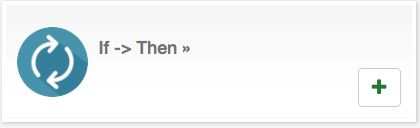
\includegraphics[width=0.4\textwidth]{pngs/cap6/app10.png}
\caption{If->Then App}
\label{app10}
\end{center}
\end{figure}

\begin{figure}
\begin{center}
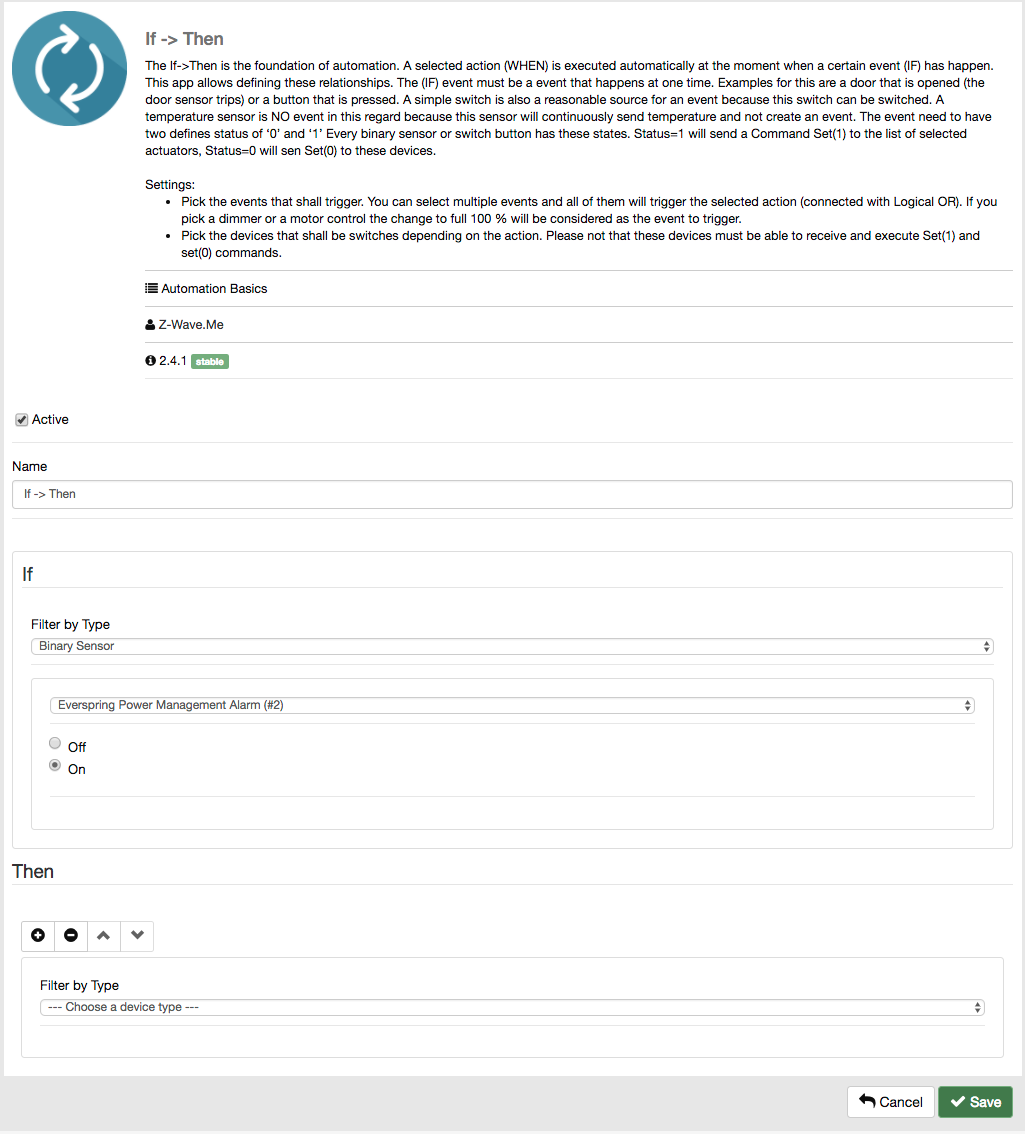
\includegraphics[width=0.4\textwidth]{pngs/cap6/app11.png}
\caption{If->Then App Configuration Dialog}
\label{app11}
\end{center}
\end{figure}

The \app{If->Then} app, as shown in Figure \ref{app10}, allows implementing the third condition, 
the relationship between event and action.

Figure \ref{app11} shows the configuration interface of the \app{If->Then} app. The first step 
is to device the event. First, select the device type of the relevant device. This will 
only shorten the list of devices (elements) to choose next. The device types are

\begin{enumerate}
\item Binary Sensor: These are typically motion detectors, smoke detectors, door sensors, but also alarm conditions of the device, e.g. power loss.
\item Binary Switch: These are all switches just knowing the state on and off.
\item Multilevel (Analog) Sensors: These are sensors measuring a certain physical value, e.g. temperature, CO2 level.
\item Multilevel Switches: These are dimmers and motor controls, e.g. for blinds or jalousies.
\item Scene Controller: These are special devices like remote control issuing special scene activation commands. The specific scene control number must be known.
\item Switch Control (On/Off/Level): These are controlling devices that report a status of the buttons, e.g. on or off.
\item Switch Control / Scene: These are controlling devices that only know one state. 
Typically, these are buttons that are pressed. The ``un-press’’ is not monitored.
\end{enumerate}

Finally, choose the event that will trigger the \app{If->Then} rule. For devices with a defined 
number of states (binary sensor, discrete sensor, binary switch, etc.), reaching this 
state is the trigger condition. Here it is enough to just pick the state (e.g. off).
For analog sensors, it must be defined if the event is reached when the measured value 
is above, equal, or below a certain trigger value.

Please note that some battery-operated sensors update their value only infrequently.
The temperature on a certain spot may rise. Unless the sensor does not transmit this 
new value, the \app{If->Then} rule will not kick in.

The second part of the configuration is defining the action. The device and action 
selection is similar to the IF part. Choose the device type first, then the specific 
device (element), and finally the action. The selection of device types differs 
from the IF section for obvious reasons:

\begin{enumerate}

\item Binary Switch: These are all switches just knowing the state on and off.
\item Color Switch: This allows changing the color on multicolor lights.
\item Door Locks:
\item Multilevel Switches: These are dimmers and motor controls, e.g. for blinds or jalousies.
\item Scene: A scene as described in Section \ref{sceneapp}
\item Thermostat: This allows defining the setpoint of a thermostat.
\end{enumerate}

Once saved, the configuration becomes active.

One special function of computers in general, and the \app{If->Then} app in particular, is that 
it does not necessarily know what the user thinks but what he configures.

Let us take an example: If the relationship is that---\textbf{IF} the door sensor is open, 
\textbf{THEN} turn on the ceiling lamp---this means that the ceiling lamp goes on when 
the door is opened. When the door is closed, the ceiling lamp will not go off because 
this was not written. If the ceiling lamp goes off, a second instance of the If->Then 
relationship is needed.
In case two devices really run synchronously with triggers on and triggers off, 
another app can realize this step instead of having two times the If->Then app. 
This app is called is called \app{Association.}


\begin{figure}
\begin{center}
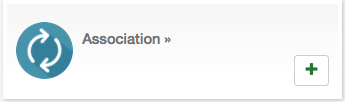
\includegraphics[width=0.4\textwidth]{pngs/cap6/app12.png}
\caption{Association App}
\label{app12}
\end{center}
\end{figure}


\subsection{Logical Rule: If->Then on steroids}


\begin{figure}
\begin{center}
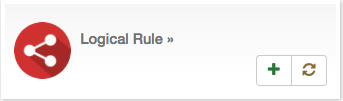
\includegraphics[width=0.4\textwidth]{pngs/cap6/app13.png}
\caption{Logical Rule}
\label{app13}
\end{center}
\end{figure}


\app{If->Then} can connect one event with multiple actions including triggering a scene with 
even more action. However, it is always one single event. For example, the night light 
will be turned on by a motion detector but only in the evening and not during the day. 
This means that different input variables need to be combined to generate the final 
scene-triggering event. The way this combination is achieved is called binary logic or 
Boolean logic, and the app implementing this is called \app{Logical Rule} as shown in 
Figure \ref{app13}. Boolean logic has three basic ways to combine variables:

\begin{itemize}
\item \textbf{AND}
\item \textbf{OR}
\item \textbf{NOT}
\end{itemize}

With these three elements, even complex relationships between variables can be described.
In case of the evening light triggered by a motion detector, the definition looks
quite simple:

\begin{center}
\textbf{IF} (it is evening) \textbf{AND} (Motion detector triggers)
$\rightarrow$
\textbf{THEN} (activate scene)
\end{center}

It is possible to connect more than two input variables using Boolean logic. However, some constrains need to be considered.

\begin{itemize}
\item The logical combinations, namely AND and OR always combine two variables. If more 
than two variables are combined, there is a need to set braces: The statement 
``A and B or C'' has two meanings: (1) always A and then either B or C, (2) Either a 
combination of A and B, or just C.

\item There is a difference between status value and events. A scene can only be 
activated by one single event, but this event can be combined with a list of status 
value. The scene is triggered only if the event happens and all the other status 
variables are in the desired status. In case a scene depends on two events, then 
the trigger condition is only true if both events happen at the same moment, 
which is quite unlikely.

A combination of variables therefore always has one single event but is not a limited 
list of other status values. Status values are ``after 17.00’’ (not right at 17.00, 
this is an event), a certain switching state of a switch (not the change of the 
switching status, this is an event).

\end{itemize}

Figure \ref{app14} shows the configuration of the \app{Logical Rule.} The first section 
allows defining certain conditions (status or events) and defines if all of them (AND) 
or just one of them (OR) will trigger the rule.

\begin{figure}
\begin{center}
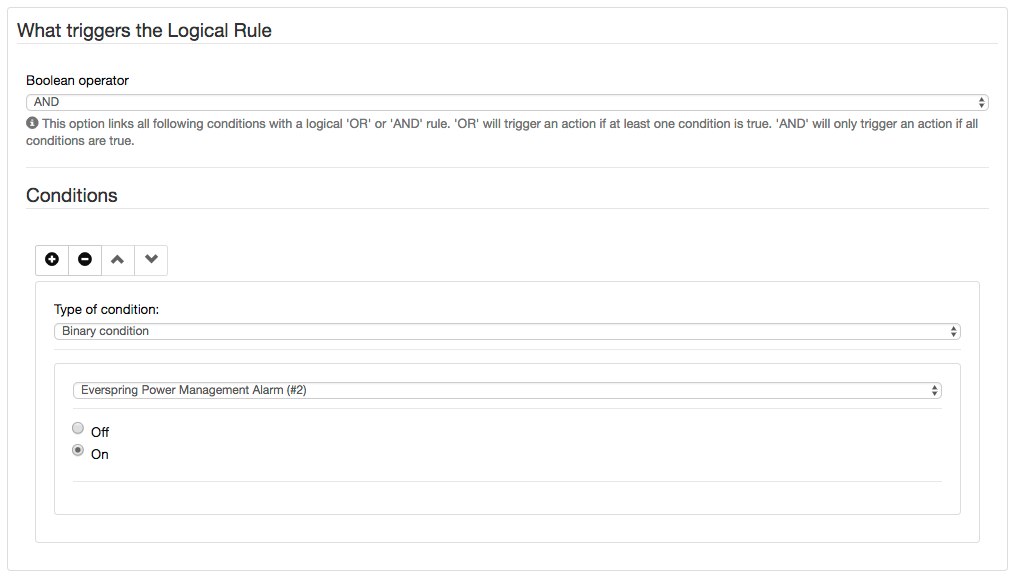
\includegraphics[width=0.4\textwidth]{pngs/cap6/app14.png}
\caption{Logical Rule}
\label{app14}
\end{center}
\end{figure}

A condition can also be the result of another combination of statuses and events. This 
is called ``nested condition,’’ which allows building a hierarchy of conditions and 
combining them in any possible way.

The action section is already known from \app{If->Then} of from scenes. The third section, 
``How the Logical Rule is triggered,’’ allows some runtime optimization.
By default, any changes in the devices mentioned in the rule will have the chance 
to trigger the entire rule. For very large rules, this may consume a lot of power. 
That’s why it is possible to limit the number of devices that can trigger the 
rule. This saves computing power.

\subsection{Tips and Tricks}

Besides the apps \app{Scene,} \app{If->Then,} \app{Logical rule,} and \app{Schedule,} there are 
a number of other apps in the app store for special automation functions. One 
little utility is worth mentioning---the dummy device shown in Figure \ref{app15}.

\begin{figure}
\begin{center}
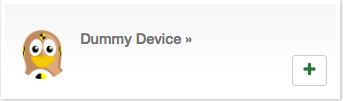
\includegraphics[width=0.4\textwidth]{pngs/cap6/app15.png}
\caption{Dummy Device}
\label{app15}
\end{center}
\end{figure}

The dummy device creates a virtual switch or dimmer that is shown as an element but does 
not have any physical function. Nevertheless, it is a valid source of events and status 
information as well as a valid device to be controlled by scenes. Sometimes, this is 
helpful to visualize certain situations in the home.


\section{The big apps}

While automation apps are more or less a toolbox to implement original ideas of certain 
automation and dependencies, the app store also offers complex apps for certain typical 
functions in the smart home that are already finished and need configuration only.

\subsection{Leakage Protection}

\begin{figure}
\begin{center}
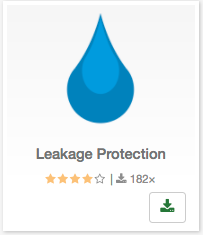
\includegraphics[width=0.3\textwidth]{pngs/cap6/app19.png}
\caption{Leakage Protection App}
\label{app19}
\end{center}
\end{figure}

The leakage protection collects all information from leakage sensors in the smart home and 
generates one single element to visualize the status of the home. Additionally, the alarm 
condition is communicated out-of-band. The app needs to be downloaded from the online 
server, as shown in Figure \ref{app19}.

\begin{figure}
\begin{center}
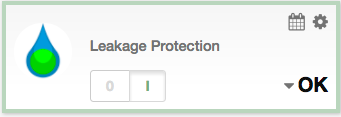
\includegraphics[width=0.4\textwidth]{pngs/cap6/app16.png}
\caption{Leakage Protection element - armed}
\label{app16}
\end{center}
\end{figure}

\begin{figure}
\begin{center}
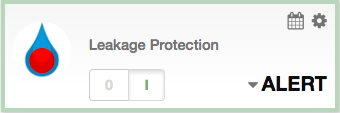
\includegraphics[width=0.4\textwidth]{pngs/cap6/app17.png}
\caption{Leakage Protection element- alarm}
\label{app17}
\end{center}
\end{figure}

\begin{figure}
\begin{center}
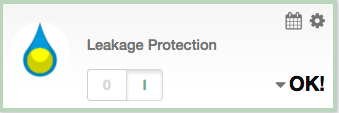
\includegraphics[width=0.4\textwidth]{pngs/cap6/app18.png}
\caption{Leakage Protection element- wait for clear}
\label{app18}
\end{center}
\end{figure}

The configuration allows picking all flood sensors in the home to trigger an alarm. In 
case of an alarm, certain actions can be triggered. The most obvious action would be to 
turn off the water supply using a Water Shut Off valve.
Additionally, it is possible to send out a notification. A drop-down list allows picking 
the desired notifier (email, push, SMS, whatever is installed) and define the message 
to send.

The app creates an element to control the leakage alarm. The element allows arming and 
disarming the system. See Figure \ref{app16} for the element when in the armed status. 
In case one of the flood detectors detects a leakage, the app will go into the alarm state:

\begin{itemize}
\item The element shows the alarm state (Figure \ref{app17}).
\item All actions defined in the configuration dialog will be executed.
\item If configured, a notification message is sent using the notifier selected.
\item The little triangle on the element allows checking which sensor triggered the alarm.
\end{itemize}

In case the alarm condition disappears (no water anymore), the alarm condition is revoked, 
but the element will show that there was an alarm event. This indication is shown in 
Figure \ref{app18}.


\subsection{Fire Protection}

\begin{figure}
\begin{center}
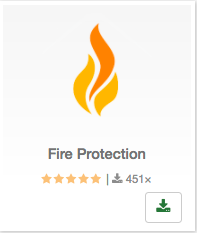
\includegraphics[width=0.3\textwidth]{pngs/cap6/app20.png}
\caption{Leakage Protection App}
\label{app20}
\end{center}
\end{figure}

The fire protection collects all information from smoke detectors in the smart home and 
generates one single element to visualize the status of the home. Additionally, the alarm 
condition is communicated out-of-band. The app needs to be downloaded from the online 
server, as shown in Figure \ref{app20}.

\begin{figure}
\begin{center}
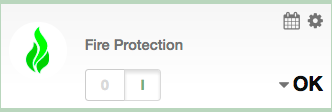
\includegraphics[width=0.4\textwidth]{pngs/cap6/app21.png}
\caption{Fire Protection element - armed}
\label{app21}
\end{center}
\end{figure}


The configuration allows picking all smoke detectors in the home to trigger an alarm. In 
case of an alarm, certain actions can be triggered. The most obvious action would be to 
turn on all lights and open the door.
Additionally, it is possible to send out a notification. A drop-down list allows picking 
the desired notifier (email, push, SMS, whatever is installed) and defines the message to send.

The app creates an element to control the fire alarm. The element allows arming and 
disarming the system. See Figure \ref{app21} for the element when in arm status. In case 
one of the smoke detectors detects a leakage, the app will go into the alarm state:

\begin{itemize}
\item The element shows the alarm state.
\item All actions defined in the configuration dialog will be executed.
\item If configured, a notification message is 
sent using the notifier selected.
\item The little triangle on the element allows checking which sensor triggered the alarm.
\end{itemize}

In case the alarm condition disappears (no water anymore), it is revoked, but the element 
will nevertheless show that there was an alarm event.

\subsection{Burglar Alarm System}


\begin{figure}
\begin{center}
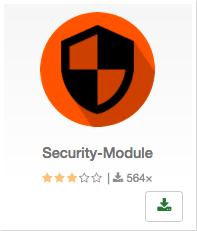
\includegraphics[width=0.3\textwidth]{pngs/cap6/app22.png}
\caption{Security System}
\label{app22}
\end{center}
\end{figure}

Security is one of the most frequently used functions of the smart home. The smart home 
can replace the traditional alarm system and implement the function using dedicated devices 
or reusing other devices such as e.g. motion detectors that were primarily installed for 
different reasons.

The app \app{Security Module} implements a complete alarm system with all the functions 
known from conventional alarm systems. The app must be downloaded from the online server, 
as shown in Figure \ref{app22}.

The configuration interface allows managing different lists of devices:

\begin{enumerate}
\item Devices that can trigger the alarm: These are all the sensors that will indicate a 
burglar in the home. These include door sensors, motion detectors, tamper switches, 
glass break sensors, etc. Per device the app allows selecting what sensor state will 
trigger the action.
\item Devices that can arm/disarm the system and clear alarms: Of course, it is possible 
to arm/disarm and clear alarms using the user interface. However, most alarm systems 
are armed/disarmed using buttons, keypads, or even smart home scenes (e.g. ``I am 
leaving home’’ or ``I am sleeping’’). For example, a simple switch can be used to arm or 
disarm the alarm system. This is not safe but doable. Per device an arm, a disarm, and 
an alarm clear status or event can be defined.
\item List of actions on alarm. This can be turning on lights, starting SONOS, switching 
a siren, and of course triggering a notification of choice.
\item List of ``arm’’ status indicators: Once the alarm system is armed, there will be 
some visible indication, besides the element on the user interface, that the house is 
armed. This could be some red lighting or some slow glowing LED light.
\item List of ``disarm’’ status indicators: Similarly, there can be devices that indicate 
that the alarm system is disarmed, e.g. with a green light.
\item List of actions when the alarm is cleared:
\end{enumerate}

The last section of the configuration allows defining time-driven arming and disarming of the system.

\begin{figure}
\begin{center}
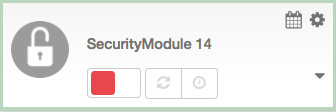
\includegraphics[width=0.4\textwidth]{pngs/cap6/app23.png}
\caption{Security System im disarm status}
\label{app23}
\end{center}
\end{figure}

\begin{figure}
\begin{center}
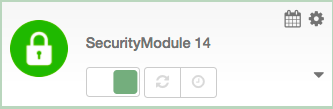
\includegraphics[width=0.4\textwidth]{pngs/cap6/app24.png}
\caption{Security System im arm status}
\label{app24}
\end{center}
\end{figure}


\begin{figure}
\begin{center}
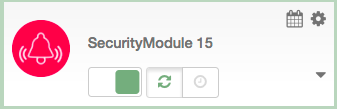
\includegraphics[width=0.4\textwidth]{pngs/cap6/app25.png}
\caption{Security System in alarm status}
\label{app25}
\end{center}
\end{figure}

The security app creates an element to control and manage the alarm system. The element 
allows arming and disarming. Figure \ref{app23} shows the alarm system in the disarm state.
 Once armed, the icon turns blue for some seconds, indicating that the alarm is turned on 
 but the alarm system is not yet fully armed. This is important as it allows users to 
 leave the home after they have armed the system.
Any sensor in the list of triggering devices will put the system in alarm state once 
triggered. This results in

\begin{itemize}
\item The element shows the alarm state with the red icon, as shown in Figure \ref{app25}.
\item All actions defined in the configuration dialog will be executed.
\item If configured, a notification message is sent using the selected notifier.
\item The little triangle on the element allows checking which sensor triggered the alarm.
\end{itemize}

Even if the triggering sensor goes back into the non-triggering state, the alarm conditions 
remain active. The alarm must be cleared by one of the devices configured or clicking on 
the alarm clear button (two arrows). The system then goes back into the arm state, as 
shown in Figure \ref{app24}. The clock icon will activate the time-driven arming and 
disarming of the alarm system.

\subsection{Climate Control}

\begin{figure}
\begin{center}
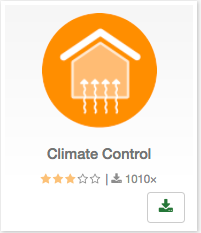
\includegraphics[width=0.3\textwidth]{pngs/cap6/app26.png}
\caption{Climate Control App}
\label{app26}
\end{center}
\end{figure}

Saving energy by having intelligent heating and climate control is one of the core values 
of the smart home. Of course, it is possible to directly control thermostats, but the 
\app{Climate Control} feature manages the whole home and offers a lot of options.

The app must be installed from the app store as shown in Figure \ref{app26}.

The climate app operates on various levels. First, there is a time-driven weekly schedule 
per room that defines the temperature in that room. The time-driven schedule should be the 
normal operation mode of the climate control feature. A second layer is the manual 
overwrite of the temperature. This overwrite can be done on a room layer as well as on the whole home layer.

The first two values are of general nature. The setback temperature is the temperature 
difference between the comfort temperature in a room and the energy-saving setback 
temperature in this room. Since different rooms may have different comfort temperatures, 
the energy-saving temperature also differs but always by the same delta. In case of doubt, 
please insert 4 Kelvin, which is a commonly accepted value.

The automation reset time defines when the normal automated heating schedule is used 
again after a manual overwrite of this schedule. The preset 2 hours is a good value.

Now there is a list of rooms. Just add your rooms you want to have the climate control 
feature. Per room you can define a temperature sensor that shows the temperature in this 
room in the climate control user interface. There is no further function of this sensor 
than showing the value in a convenient way. Please note that the dropdown list will 
only show temperature sensors that are assigned to this room. The comfort temperature 
is the room-specific temperature. Usually it is higher in bathrooms than in sleeping 
rooms. Your individual preference matters here.


\begin{figure}
\begin{center}
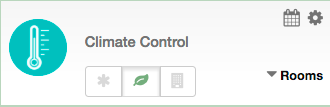
\includegraphics[width=0.3\textwidth]{pngs/cap6/app27.png}
\caption{Climate Control App Element}
\label{app27}
\end{center}
\end{figure}

The last section of the configuration dialog is the heating schedule. It allows setting a 
temperature at certain time slots on certain days per week for certain rooms.

As shown in Figure \ref{app27}, the app generates a special element. It allows running the 
climate control for the whole home in three basic modes:

\begin{itemize}
\item 
\includegraphics[width=0.04\textwidth]{pngs/cap6/app27a.png} The heating in the home 
is turned off. This will overwrite all schedules and all settings in every room.
\item 
\includegraphics[width=0.04\textwidth]{pngs/cap6/app27b.png} The heating in the 
whole home is in the energy-saving mode. This will overwrite all schedules and all settings per room.
\item 
\includegraphics[width=0.04\textwidth]{pngs/cap6/app27c.png} No home-wide 
overwrite. The room-specific settings apply.
\end {itemize}

The little triangle on the right-hand side allows opening the room view as shown in 
Figure \ref{app27d}. Here, it is possible to see the actual temperature per room plus the 
current desired temperature. A dropdown list allows choosing the heating mode for 
the specific room:

\begin{figure}
\begin{center}
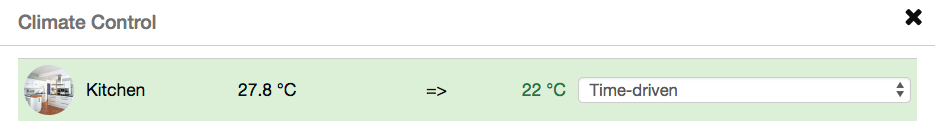
\includegraphics[width=0.3\textwidth]{pngs/cap6/app27d.png}
\caption{Climate Control App Element - room view}
\label{app27d}
\end{center}
\end{figure}

\begin{itemize}
\item \textbf{Frost Protection:} The room is in the frost protection state (around 8 degrees C).
\item \textbf{Energy Save:} The room is in the energy-saving state. This is the comfort 
temperature minus the setback temperature difference defined in the configuration dialog.
\item \textbf{Comfort:} The room is in comfort temperature as defined in the configuration dialog.
\item \textbf{Time driven:} The heating schedule as defined in the configuration dialog applies.
\end {itemize}

\section{Out-of-band notifications}

All events in the smart home are shown in the user interface, or they can be indicated 
using devices inside the home. However, people do not always monitor the user interface. 
Hence, there are the so-called out-of-band notification options to reach the user in such a case:

\begin{itemize}
\item Email
\item SMS
\item Push notifications right on the home screen of the mobile phone
\item voice call
\end{itemize}

\zway supports various ways of out-of-band communication. For every communication channel, 
multiple apps from different providers may exist to realize the same function. However, 
all these notifiers work in the same manner:

\begin{itemize}
\item They establish an out-of-band communication channel.
\item They need to be configured according to the user’s preferences.
\item They accept messages from other apps and forward them as configured.
\item They create an element with a push button to send a simple test message.
\end{itemize}

Some out-of-band notifiers make it possible to gather and filter events from the timeline 
and forward them. This must be configured in the configuration dialog.

\subsection{Push Notifications}

Push notifications are delivered to a mobile phone. As soon as one of the native Z-Wave.Me 
apps is installed on the mobile phone, the push notification option is automatically 
enabled. Push notifications allow gathering events and forwarding them automatically. This 
can be configured in the apps \app{Mobile Phone Support, Notification Filtering} which is already running in the 
system. Please go to \keystroke{Active} app management to open the configuration dialog.

\subsection{Notifications by E-mail}

\begin{figure}
\begin{center}
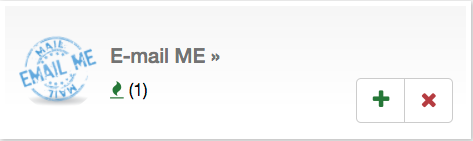
\includegraphics[width=0.3\textwidth]{pngs/cap6/app31.png}
\caption{Notifications by E-mail}
\label{app31}
\end{center}
\end{figure}

The \app{Notifications by E-mail} app, as shown in Figure \ref{app31}, for each user creates a communication channel for sending events by email.

In the \app{Notification Filtering} application, you can select the notification channel, it can be email, push, sms or a channel provided by third-party applications: facebook, twitter and others. 

\subsection{Other notifiers}

Besides the two standard notifiers for push notifications and email, the app store has 
plenty of other notification apps from third-party developers. Just check out what works for you.

\section{Useful tools and utilities}

The app store is a gold mine of cool applications. This manual can only mention a few of 
the more popular ones. Of course, you can check out the display of apps according to popularity, etc.

\subsection{Apple HomeKit}

As shown in Figure \ref{app40}, the Apple Home Kit App, provided by a third-party programmer 
named Andreas Freud, connects \zway with Apple’s HomekitWorld. Once installed, the \zway 
controller is shown to Apple as a Homekit bridge device. Please be aware that this app is 
maintained by a third-party developer and the existence of the apps is certainly not in 
the main interest of Apple.

\begin{figure}
\begin{center}
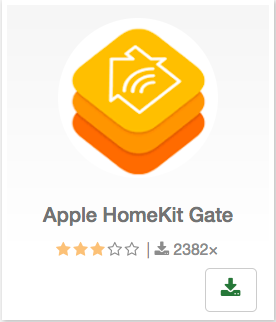
\includegraphics[width=0.3\textwidth]{pngs/cap6/app40.png}
\caption{Apple Homekit Integration}
\label{app40}
\end{center}
\end{figure}

\subsection{Intchart.com}


\begin{figure}
\begin{center}
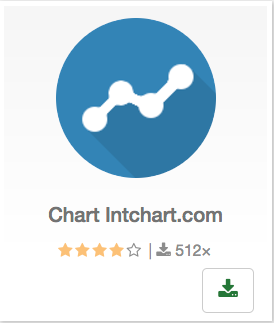
\includegraphics[width=0.3\textwidth]{pngs/cap6/app41.png}
\caption{Intchart.com Integration}
\label{app41}
\end{center}
\end{figure}

This app (Figure \ref{app41}) adds a little icon to the selected device. Clicking on this 
icon opens a window with a chart showing its history. To use this app, you have to be 
registered at www.intchart.com. Note that if you change the settings below, the chart can 
be reset, but the previous chart will still be visible on intchart.com.

The settings are as follows:

\begin{itemize}
\item First, register at www.intchart.com.
\item Below that, select the devices to track.
\item Indicate if they have to be on the same chart.
\item Indicate if you want to have a difference between values (for energy consumption, etc.).
\item Choose the poll period.
\item Paste the API user ID and API key from your account: www.intchart.com.
\end{itemize}


\subsection{Astronomy App}


\begin{figure}
\begin{center}
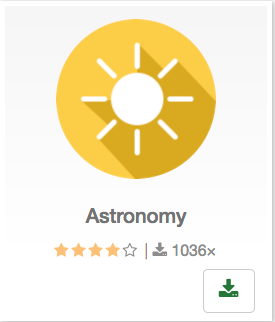
\includegraphics[width=0.3\textwidth]{pngs/cap6/app42.png}
\caption{Astronomy App}
\label{app42}
\end{center}
\end{figure}

This app (Figure \ref{app42}) from  Maros Kollar calculates the position 
of the sun above the horizon for the given location. The module provides various metrics 
for other automation modules like sun altitude and azimuth, and emits events when the sun 
reaches certain positions. This module can be used to control light scenes or shading 
based on the solar position.

Check github.com/maros/Zway-Astronomy for detailed documentation.


\subsection{Alexa Integration}

This app in Figure \ref{app43} integrates \zway with the Amazon Alexa Voice Control system. 
Once installed, you need to activate the ``skill’’ in the Alexa user interface before using.

\begin{figure}
\begin{center}
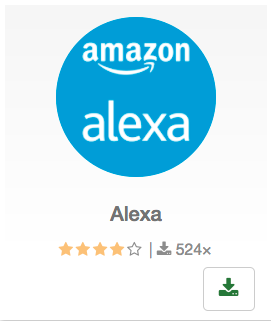
\includegraphics[width=0.3\textwidth]{pngs/cap6/app43.png}
\caption{Amazon Alex Integration}
\label{app43}
\end{center}
\end{figure}

\subsection{Philips Hue Integration}


HUE is a new way to use your Philips Hue SmartHome solutions. Use this app (Figure \ref{app44}) 
as a remote to  switch colors, turn up the brightness, and quickly toggle between lights on 
and off. For the moment, you have to create your credential manually.

Installation instructions:

\begin{itemize}
\item Go to http://YourBridgeIpAddress/debug/clip.html
\item Enter \{\"devicetype\":\"SmartHome\#RasberryPi Zway\"\} in MessageBody part.
\item Go and press the button on the bridge.
\item Press the POST button on clip.html page and you should get a success response.
\item Congratulations you have just created an authorized user (like: 1028 d66426293e821ecfd9ef1a0731df), which we’ll use from now on.
\item Fill your key in the Hue app!
\end{itemize}

To create your own key, see more details on:
\begin{itemize}
\item www.developers.meethue.com/documentation/getting-started
\item https://github.com/timauton/Hue
\end{itemize}
\begin{figure}
\begin{center}
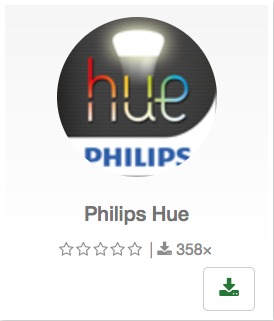
\includegraphics[width=0.3\textwidth]{pngs/cap6/app44.png}
\caption{Philips Hue Integration}
\label{app44}
\end{center}
\end{figure}


\section{For Developers}

\begin{figure}
\begin{center}
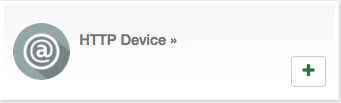
\includegraphics[width=0.3\textwidth]{pngs/cap6/app28.png}
\caption{HTTP device}
\label{app28}
\end{center}
\end{figure}

Apps for developers require a certain amount of programming skills and partly require 
knowledge about the \zway data model. Please refer to Chapter \ref{c:developer} for details.

Nevertheless, the app \app{HTTP} device allows adding certain functions without deep 
software knowledge. The \app{HTTP} device generates a sensor or an actor depending on 
information obtained by just accessing a website using HTTP.

One example will demonstrate this. The goal is to make an element that shows the current 
USD/EUR exchange rate. The website 

\murl{http://api.fixer.io/}

offers this data free of charge. Even more conveniently, the URL 

\murl{http://api.fixer.io/latest} 

delivers information in a 
machine-readable JSON format (you can use the URL in a standard web browser to have a 
look at the structure.)


In the http device configuration, a multilevel sensor is chosen, since only values 
have to be shown and they are not only 0 and 1. Then the URL api.fixer.io is provided 
(attention, without http!). This will now call the whole JSON data set. For the element, 
the right value needs to be extracted. Here some JavaScript knowledge is needed to 
understand the command 

\cmdline {``\$\$.rates.USD.’’ }

Finally, the refresh rate is defined and a 
nice name given. The other form elements are not needed here.
After saving the configuration, the new element is visible. A little optimization is to 
show the cent value by changing the JavaScript into 

\cmdline{``parseFloat(\$\$.rates.USD)*100.’’}

The sensor based on the exchange rate can now be used like any other analog sensor. 
Setting a trigger on certain exchange rates may be used to activate a special scene. 
Indeed, this is more for day traders on EUR/USD exchange, but may still be cool.


\begin{figure}
\begin{center}
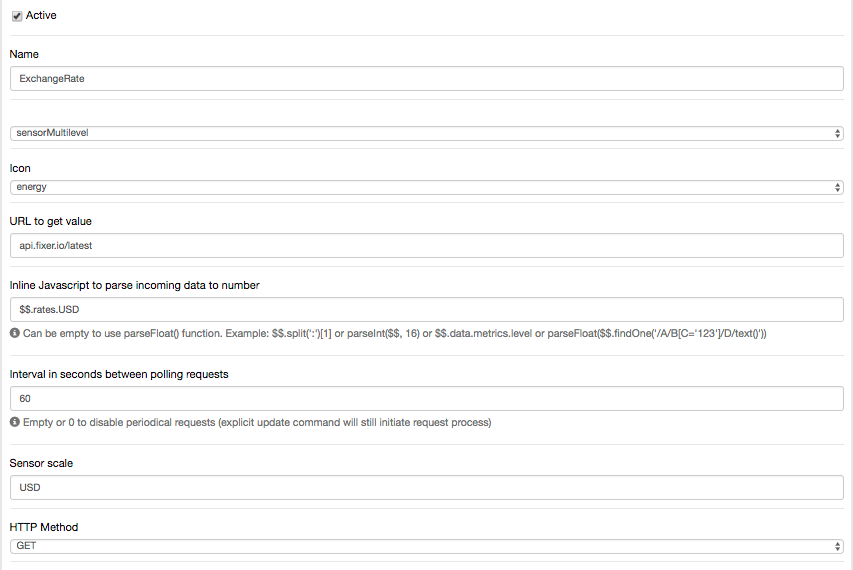
\includegraphics[width=0.9\textwidth]{pngs/cap6/app29.png}
\caption{HTTP device - Configuration dialog for currency exchange ``sensor’’}
\label{app29}
\end{center}
\end{figure}

\begin{figure}
\begin{center}
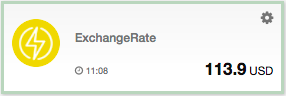
\includegraphics[width=0.3\textwidth]{pngs/cap6/app30.png}
\caption{Currency Exchange Element}
\label{app30}
\end{center}
\end{figure}
